\chapter{Participation at the Global Doc Project}
During his PhD the author of the present work spent a five month interchange period in Italy, at the Università degli Studi di Bari Aldo Moro (UNIBA) located in Bari (Puglia region). The interchange was funded by the UNIBA through the Global Doc project, which was developed to promote the local interaction of PhD students, from several countries around the world and different research fields, with the UNIBA local community. This interchange allowed the author to be very close to his co-advisor since the Physics department of UNIBA (Dipartimento Interateneo di Fisica Michelangelo Merlin) sits at the same campus where is located the INFN and Politecnico di Bari. This period abroad also allowed the author to personally participate of two very good events: the Electroweak Symmetry Breaking Spring school (EWSB)\footnote{EWSB school: \url{https://indico.cern.ch/event/673580/}.} and the Monte Carlo net school (MCnet)\footnote{MCnet school: \url{https://indico.cern.ch/event/669309/}.}.

The period spent at UNIBA was also very productive for the author. Differently from the period spent at Fermilab as visiting scientist, the Global Doc project promoted the interaction of the author with several (PhD, Master and Grad) students (even another Brazilians) from different research fields. This is a good scenario for interchange of ideas, which finally achieved his apex during the Global Doc Seminars section. In this seminar each student enrolled in the project had to give a presentation about his (her) research field, allowing the students to expose their work and receive questions from very different view angles. Fig.~\ref{fig:global_doc_seminar} shows some picture from the seminar given by the author at UNIBA.

\begin{figure}[htbp]{16cm}
	\caption{Some pictures of the seminar given by the author at UNIBA during his participation in the Global Doc project. The organizers, the local tutor prof. Giovanna Selvagi and the co-advisor prof. Nicola were present in the seminar, which was also opened to the university academic community.}
	\centering
	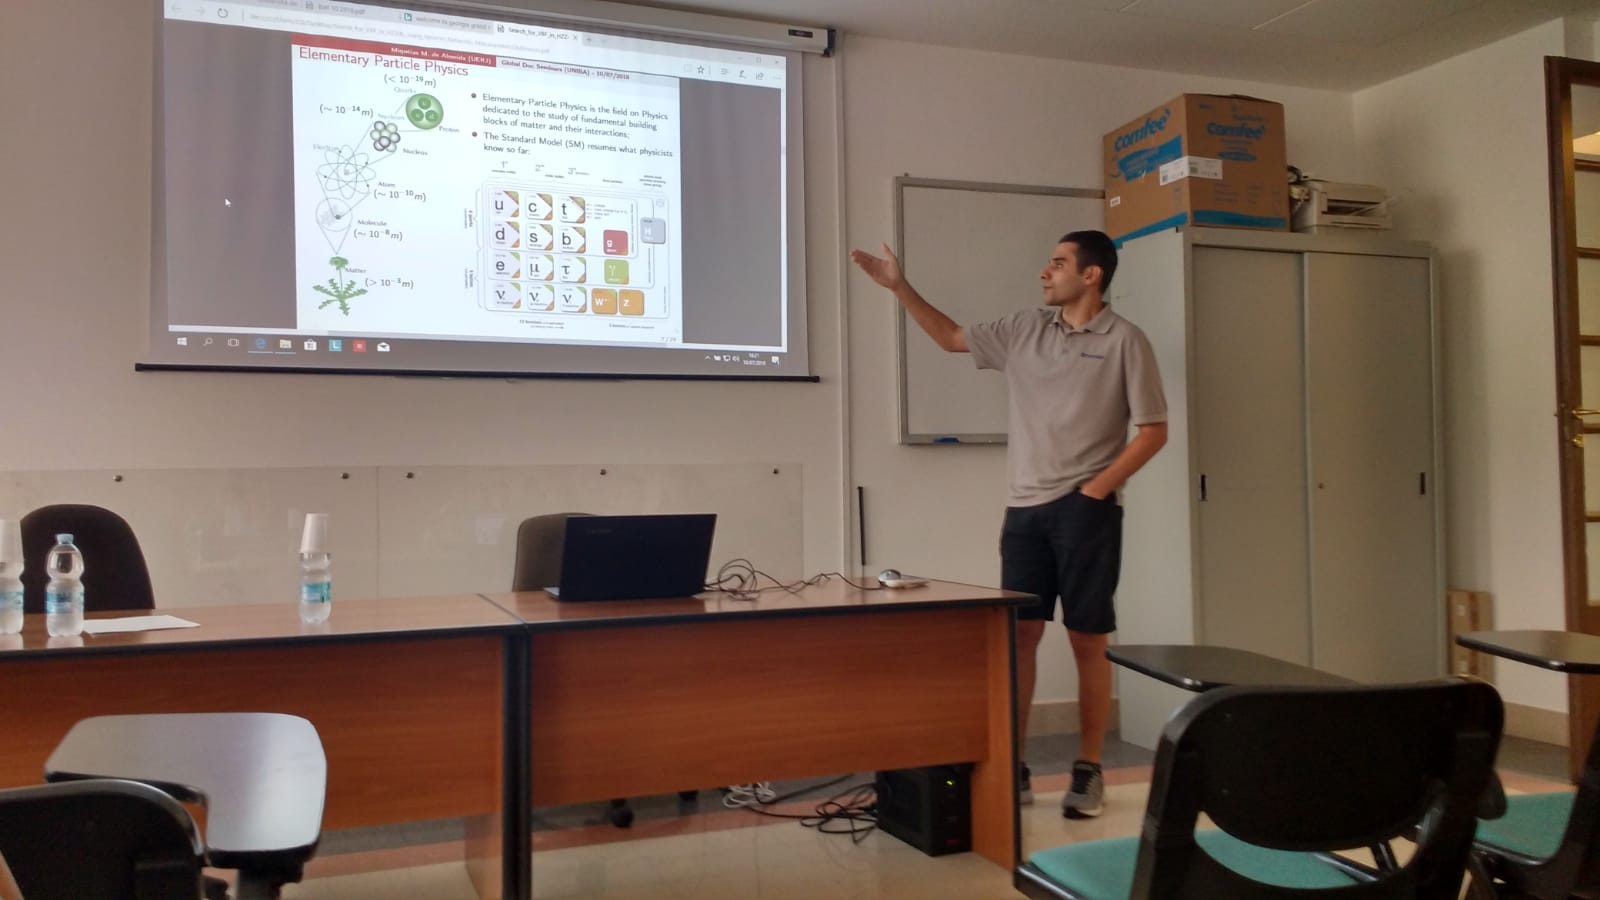
\includegraphics[width=12cm,height=7cm,trim={0cm 0cm 0cm 0cm},clip]{AppendixGlobalDocProject/figs/miqueias_globaldoc_seminar2}\\
	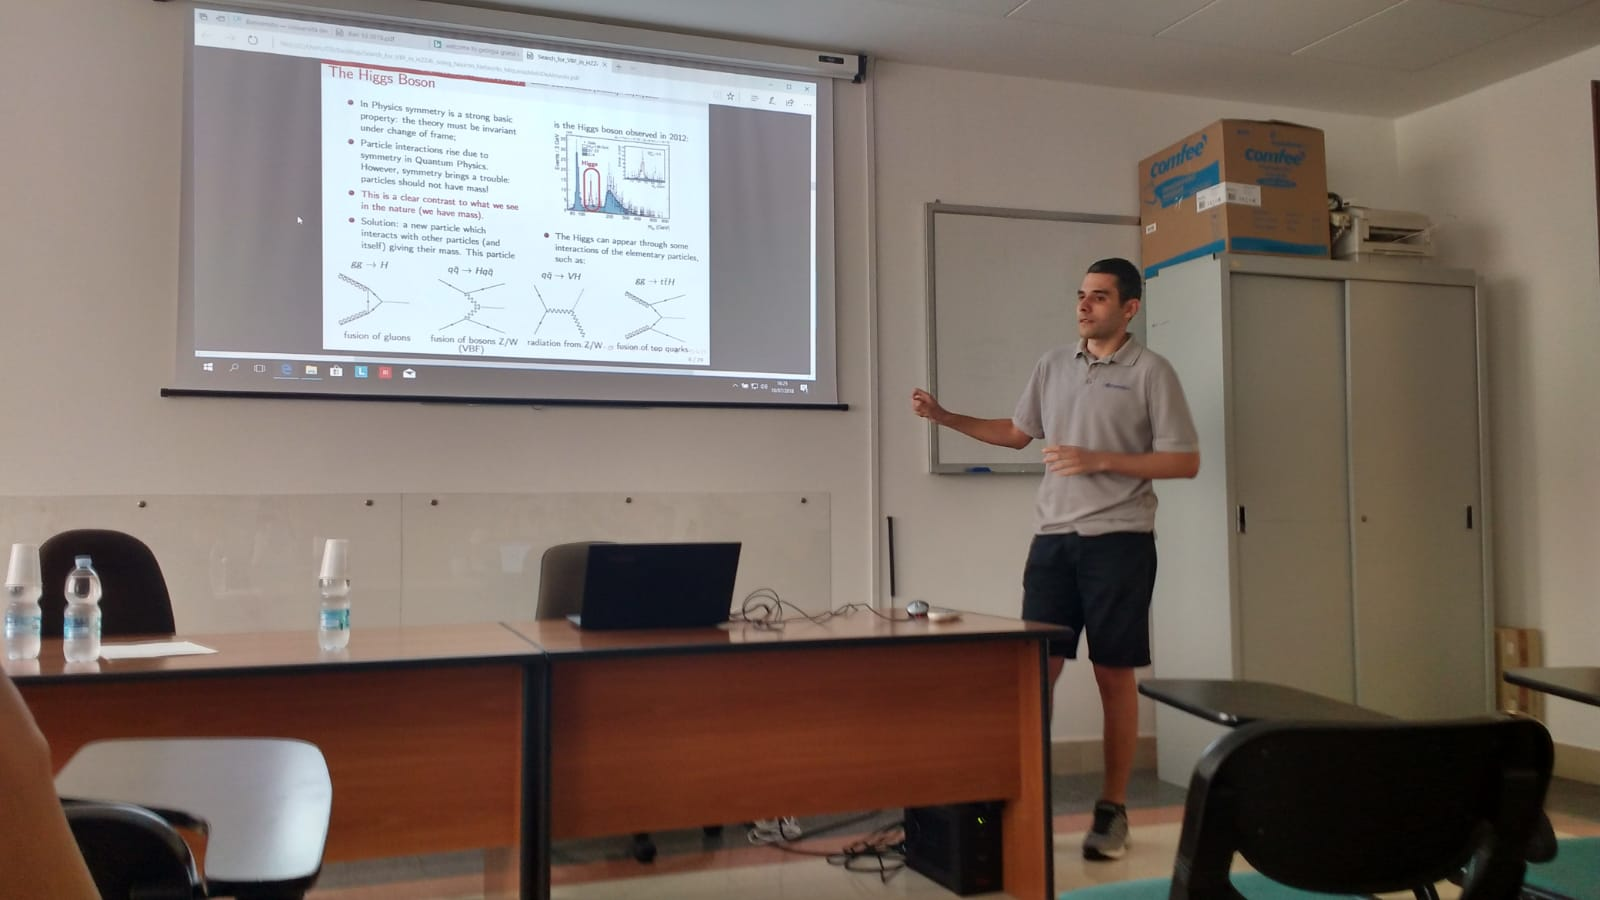
\includegraphics[width=12cm,height=7cm,trim={0cm 0cm 0cm 0cm},clip]{AppendixGlobalDocProject/figs/miqueias_globaldoc_seminar1}\\
	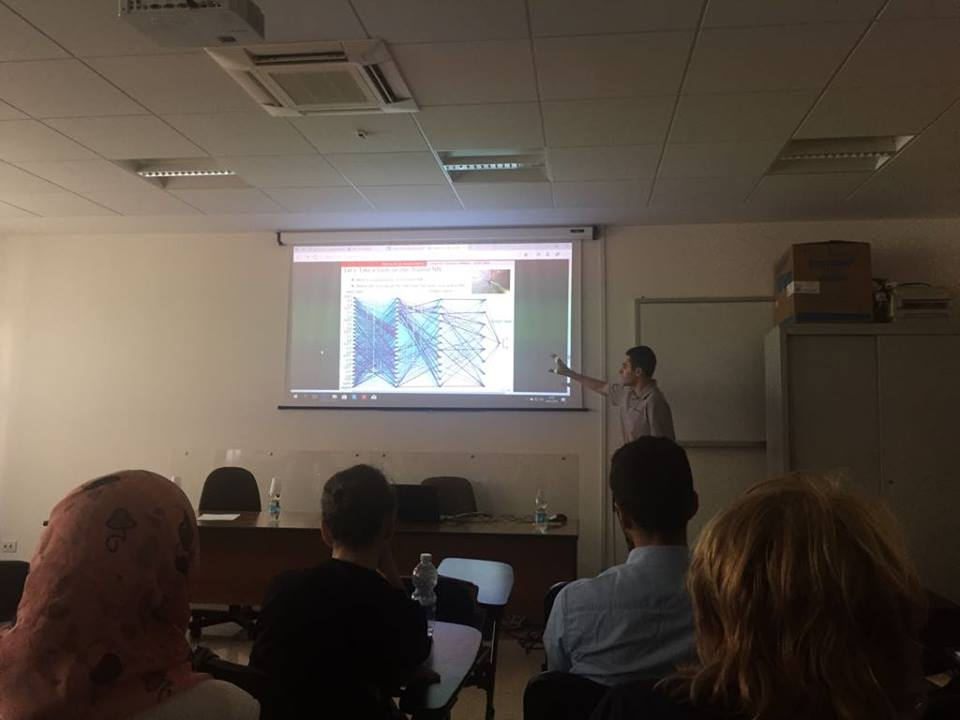
\includegraphics[width=12cm,height=7cm,trim={0cm 0cm 0cm 2cm},clip]{AppendixGlobalDocProject/figs/miqueias_globaldoc_seminar}
	\source{The AUTHOR, 2018.}
	\label{fig:global_doc_seminar}
\end{figure}

In terms of the Physics, the period spent at UNIBA brought good experiences for the author. One of the main impacts was the development of the strategy to estimate the systematic uncertainties associated to the VBF ANN discriminants due to their inputs. That demanded the re-processing of MC samples used in this present analysis which was possible by using the computer farm RECAS\footnote{Details here: \url{https://www.recas-bari.it/index.php/it/}.} at UNIBA Fig.~\ref{fig:recas_cluster}. This procedure has been also important for another analysis about Dark Matter leaded by the author's co-advisor. Because of that, the author spent also some time in that analysis contributing on the final systematic uncertainties estimation and on the statistical analysis through the advanced features contained into Higgs Combine tool. This was a good experience for the author which applied similar studies to work presented in this thesis. 

\begin{figure}[htbp]{16cm}
	\caption{The RECAS computing farm at the UNIBA campus where the Physics department is located.}
	\centering
	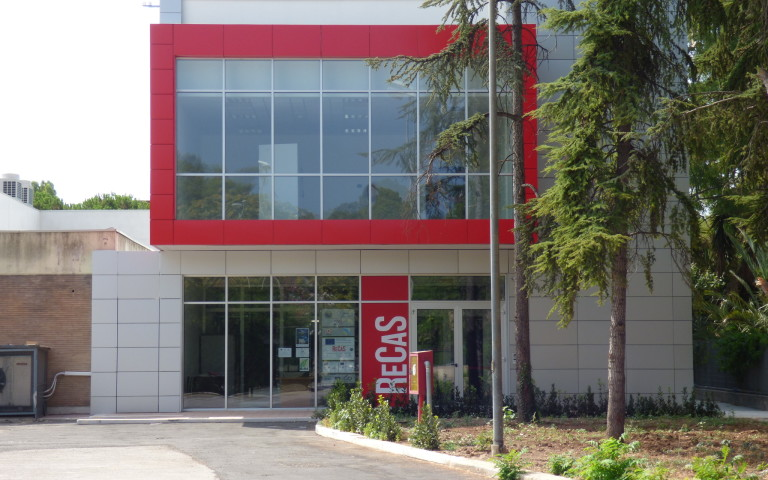
\includegraphics[width=12cm,height=7cm,trim={0cm 0cm 0cm 0cm},clip]{AppendixGlobalDocProject/figs/recas_bari}\\[0.5cm]
	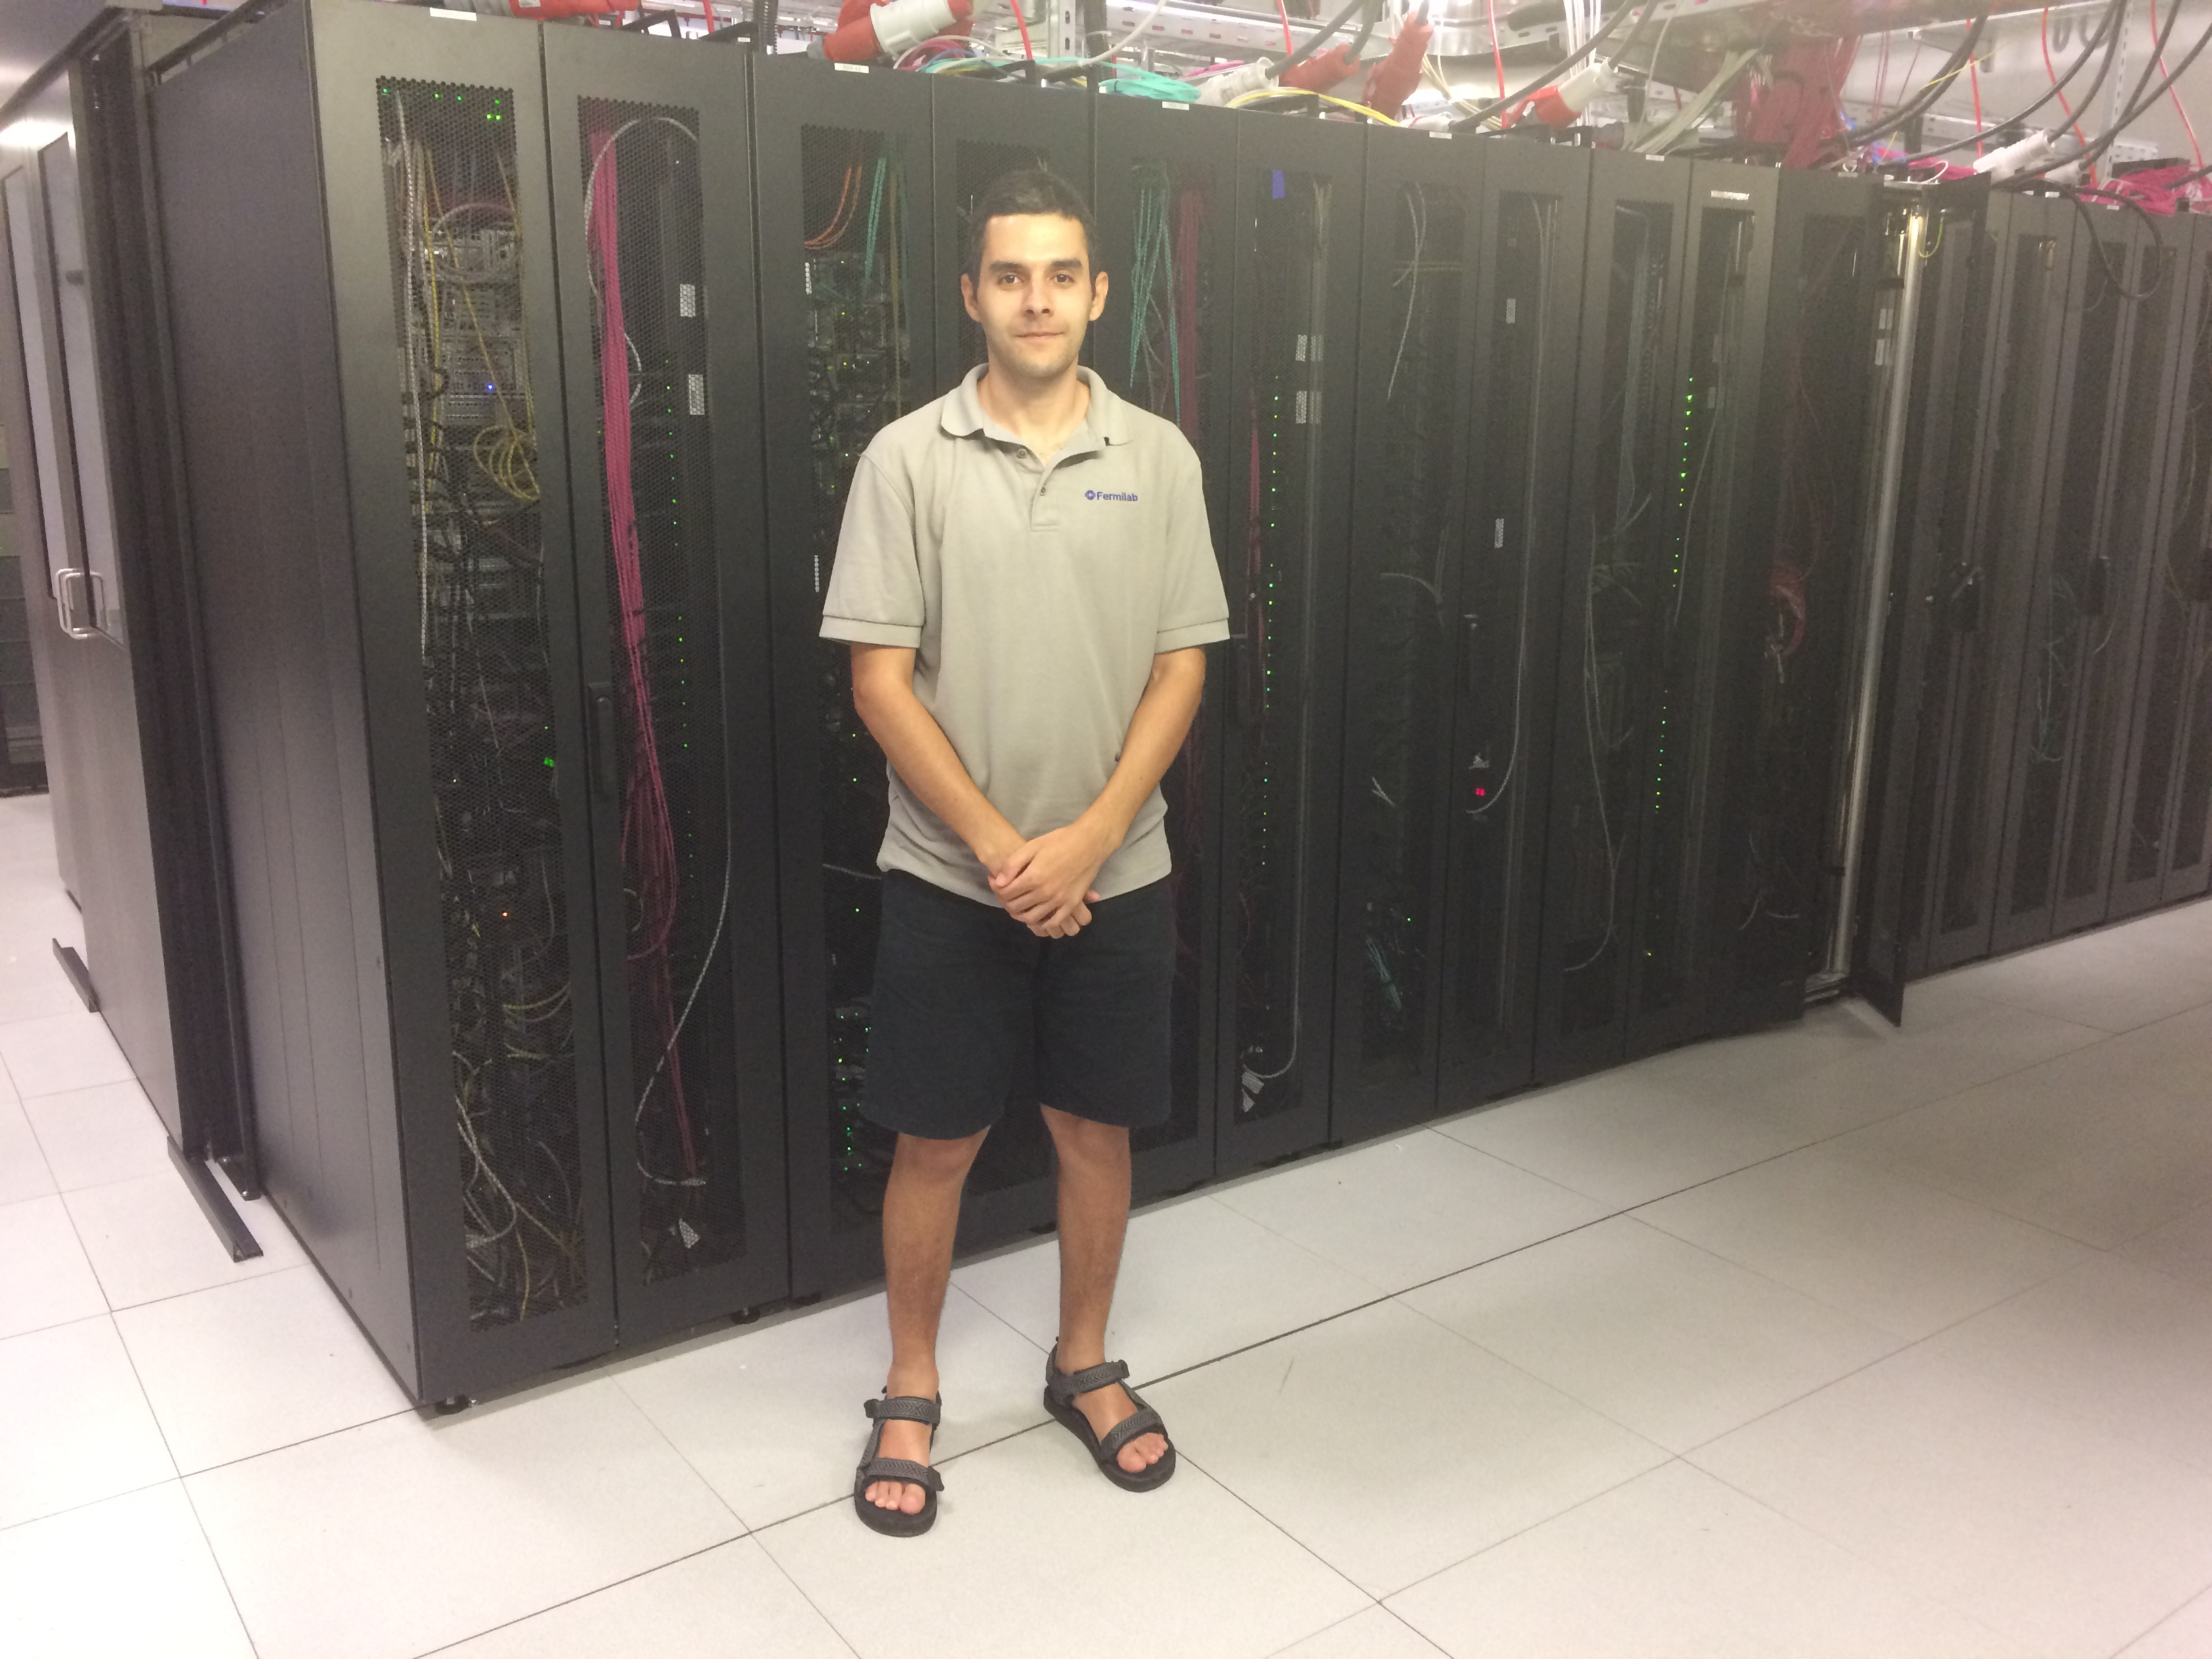
\includegraphics[width=12cm,height=9cm,trim={0cm 0cm 0cm 0cm},clip]{AppendixGlobalDocProject/figs/miqueias_at_recas}
	\source{The AUTHOR, 2018.}
	\label{fig:recas_cluster}
\end{figure}

This Dark Matter analysis is essentially based on the search for Dark Matter candidates associated to Higgs production mechanisms (Higgsstrahlung) as shown in Fig.~\ref{fig:dm_plots}(a). The Dark Matter candidate in this case is the $Z'$ boson from two models. This particle appears in simplified models extending the SM gauge group with new symmetries, which in the referring analysis are the 2HDM (Two Higgs Doublet Model) and the Baryonic. In the 2HDM model the $Z'$ decays into a Higgs (SM or not) and a neutral pseudoscalar particle $A^{0}$. In the Baryonic model the $Z'$ irradiates a Higgs (not SM). In both models there is MET in the final state due to the decay of the $A^{0}$ or $Z'$ into a pari $\chi\bar{\chi}$ (neutralinos - supersymetrical partners of neutrinos). Hence, the analysis is ultimately done over the MET distribution which is very sensitive for discriminate SM processes from these Dark Matter candidate process, see Fig.~\ref{fig:dm_plots}(b). For more details about this analysis, please see \cite{bib:CMS-AN-16-328}.

\begin{figure}[htbp]{16cm}
	\caption{Briefly of the Dark Matter analysis: (a) the LO diagrams of the searched processes and (b) the MET distribution (stacked) for SM processes and (superimposed) Dark Matter candidates.}
	\centering
	\subfloat[]{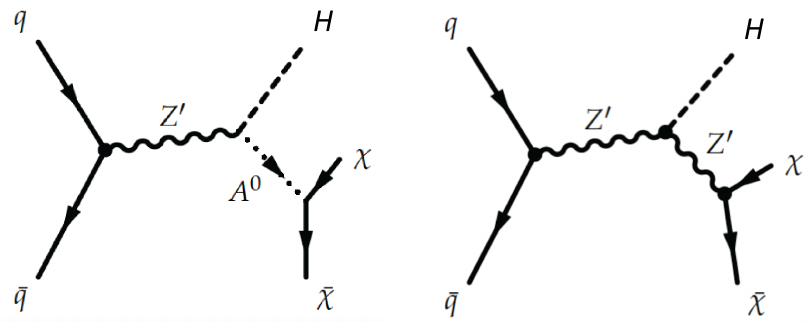
\includegraphics[width=7cm,height=4cm,trim={0cm 0cm 0cm 0cm},clip]{AppendixGlobalDocProject/figs/dm_diagrams}}\quad\quad
	\subfloat[]{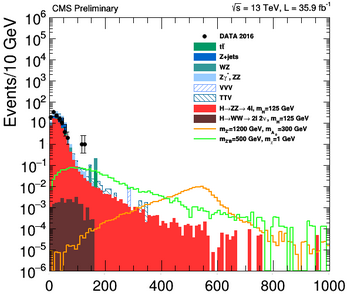
\includegraphics[width=6cm,height=4cm,trim={0cm 0cm 0cm 0cm},clip]{AppendixGlobalDocProject/figs/met_plot}}
	\source{Refference \cite{bib:CMS-AN-16-328} p. 10 and adapted from \cite{bib:CMS-AN-16-328} p. 49.}
	\label{fig:dm_plots}
\end{figure}

Another experience at UNIBA for the author, though shortly, has been the guiding of another student of the author's co-advisor through some basics on the MadGraph MC generator. This student was developing his PhD research project on the double and triple Higgs production processes, aiming the study of the associated couplings.

Finally, a very briefly documentation of each student participating in the Global Doc has been prepared and presented by the organizers of the project at the \textbf{Verso Horizon 2012-2017. La ricerca in rete in Europa}\footnote{See:  \url{https://www.uniba.it/eventi-alluniversita/2018/verso-horizon-europe-2021-2027}.} congress, which happened on October 5th, 2018 at the UNIBA. For the interested reader, please see \url{https://www.uniba.it/elenco-siti-tematici/altri-siti-tematici/globaldoc}, which is the Global Doc web page and where one can find detailed information on this project and about future selective processes. According to the organizers, the documentation about the students participation on the project will be attached to that web page in the future.